Con el desarrollo de la librería ya es posible hacer la implementación de un proyecto el cual ya usa React.
A continuación se ejemplifica el uso de la librería paso a paso.

Existe una herramienta que nos permite crear el esqueleto de una web basada en React. \cite{CRA} esta es desarrollada y mantenida por Facebook, de la cual partiremos para crear una web en la que probaremos la librería.

Instalaremos la herramienta llamada Create React App con el siguiente comando.
\newline
\begin{figure}[H]
    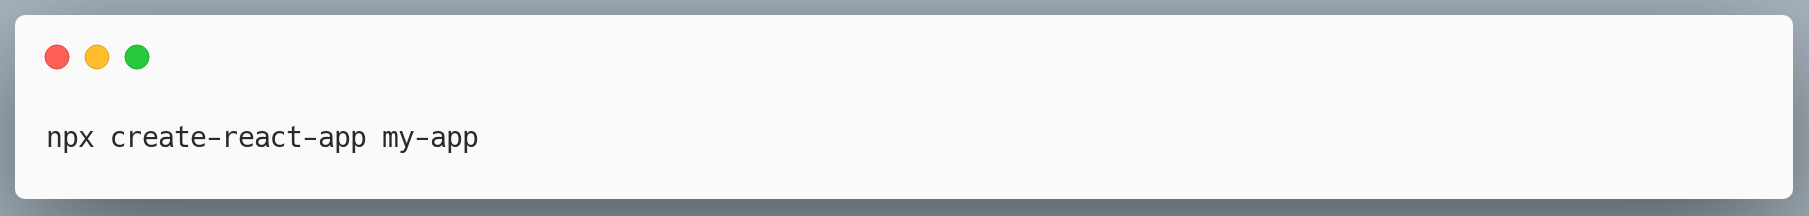
\includegraphics[width=1\textwidth]{./Imagenes/9.1.png}
    \caption[Instalar Create React App]{Instalar Create React App}
    \end{figure}
\newline

Crearemos la web llamada ejemplo-1 con el siguiente comando.
\newline
\begin{figure}[H]
    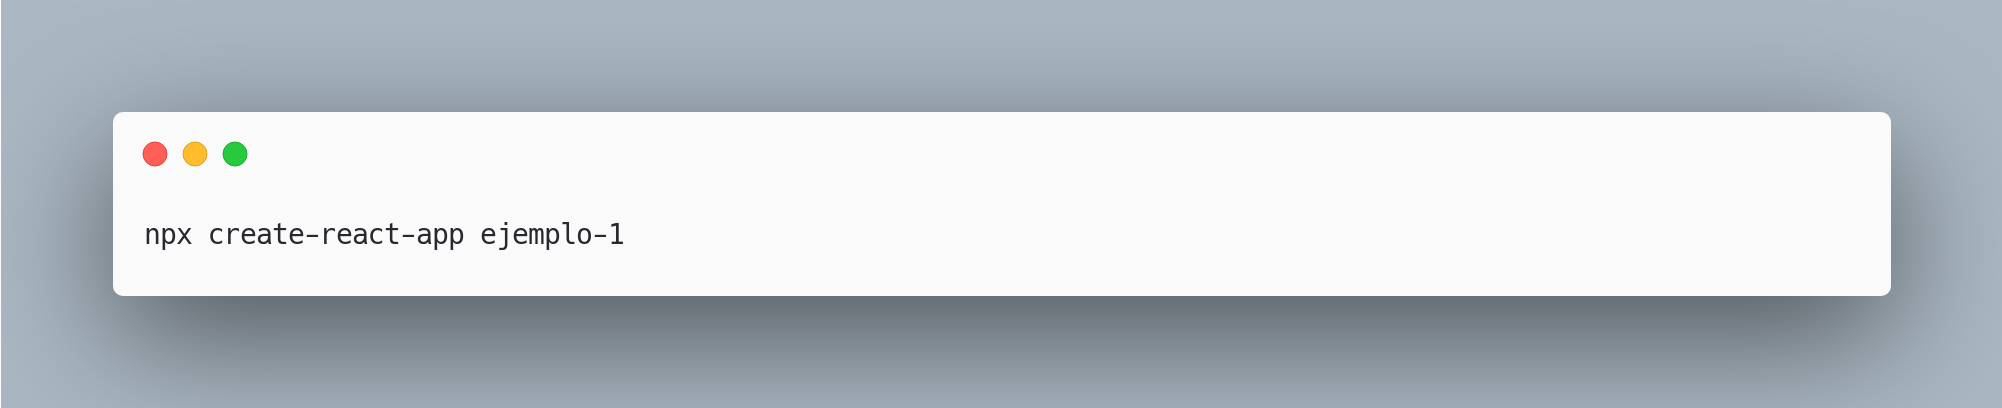
\includegraphics[width=1\textwidth]{./Imagenes/9.2.png}
    \caption[Crear una nueva app]{Crear una nueva app}
    \end{figure}
\newline

El comando nos generará los siguientes directorios.
\newline
\begin{figure}[H]
    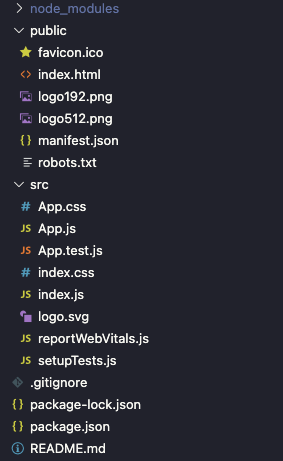
\includegraphics[width=0.5\textwidth]{./Imagenes/9.3.png}
   \centering 
    \caption[Directorios al crear una nueva app]{Directorios al crear una nueva app}
    \end{figure}
\newline

Para poder probar nuestra librería debemos a indicar a la app ejemplo-1 que use la dependencia instalándola con el siguiente comando.\newline
\newline
\begin{figure}[H]
    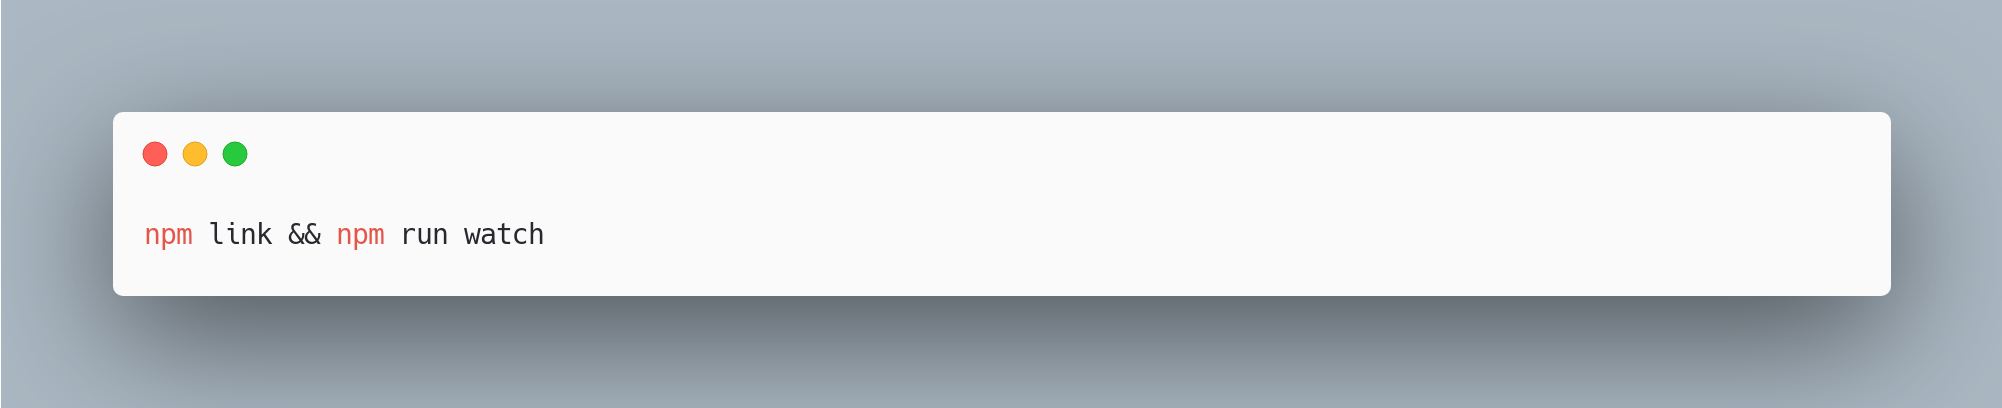
\includegraphics[width=1\textwidth]{./Imagenes/9.4}
   \centering 
    \caption[Instalando nuestra librería]{Instalando nuestra librería}
    \end{figure}
\newline

Ahora basta incluirlo como se agrega cualquier dependencia de node, basta con agregar cualquiera de los elementos aquí desarrollados. 

Crearemos dos ejemplos simples para mostrar el funcionamiento de la librería.
El primero consta de un formulario el cual solicita nombre, correo electronico y contraseña, esto con el objetivo de registrar un usuario para que tenga un correo institucional, también se le solicitará si la cuenta estará activa al momento de crearla.

Para esto debemos importar nuestros componentes de la siguiente manera.
\newline
\begin{figure}[H]
    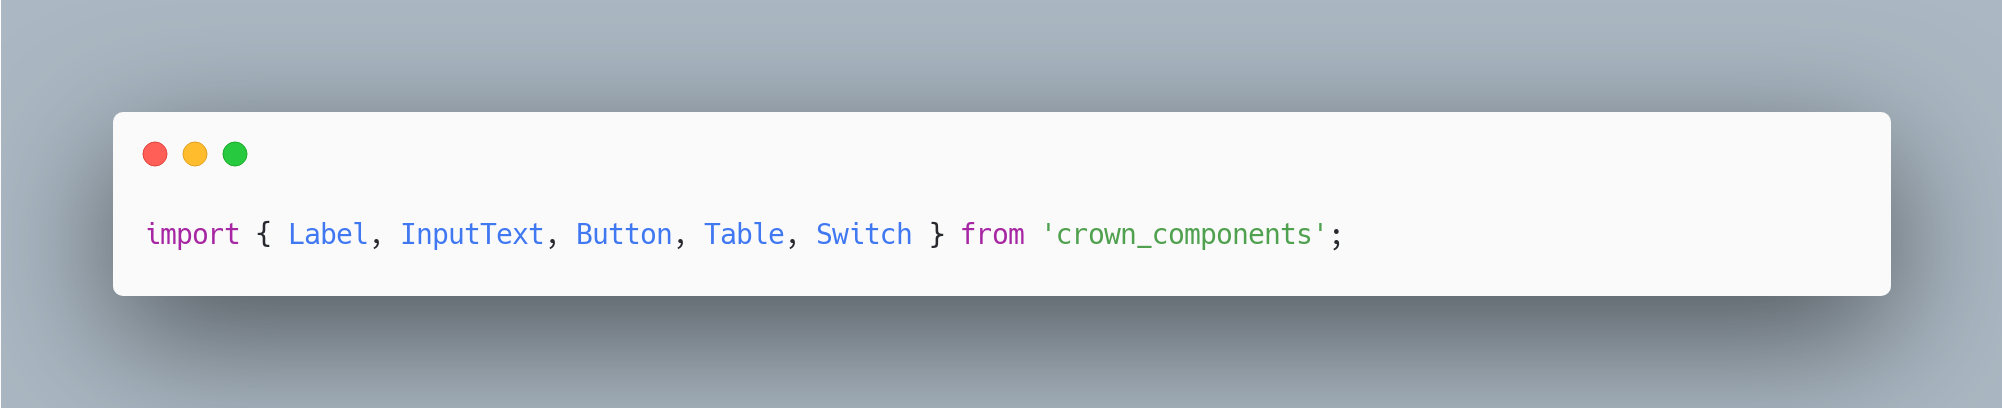
\includegraphics[width=1\textwidth]{./Imagenes/9.6}
   \centering 
    \caption[Implementación la librería]{Implementación la librería}
    \end{figure}
\newline

Después en el estado de React debemos agregar algunos campos para almacenar la información del formulario como se muestra en la siguiente figura.
\newline
\begin{figure}[H]
    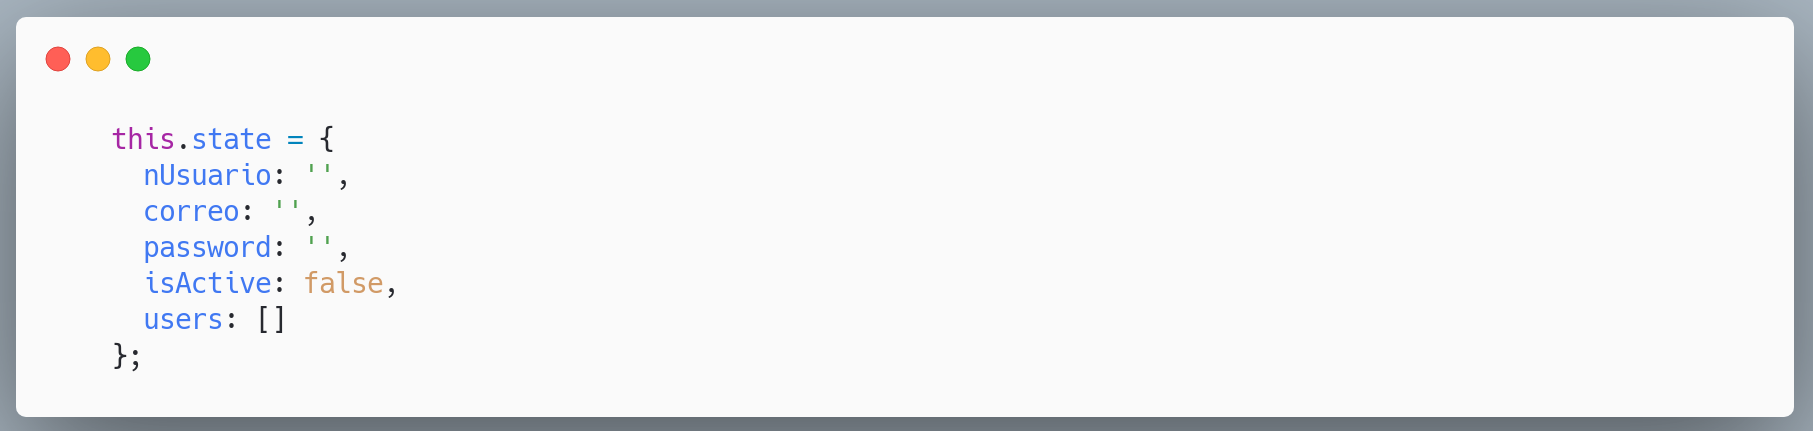
\includegraphics[width=1\textwidth]{./Imagenes/9.7}
   \centering 
    \caption[Agregar campos al estado de React]{Agregar campos al estado de React}
    \end{figure}
\newline
Los datos se usarán para:

  \begin{itemize}
   \item \textbf{ nUsuario:} Nombre de usuario del nuevo registro.
   \item \textbf{ correo:} Correo del usuario.
   \item \textbf{ password:} Contraseña del usuario.
   \item \textbf{ isActive:} Activar la cuenta al crearla.
   \item \textbf{ users:} Usuarios registrados, esto simulando nuestra base de datos.
  \end{itemize}

En la siguiente imagen se muestra el código necesario para desplegar en pantalla el formulario requerido así como una tabla para mostrar los usuarios registrados.

\newline
\begin{figure}[H]
    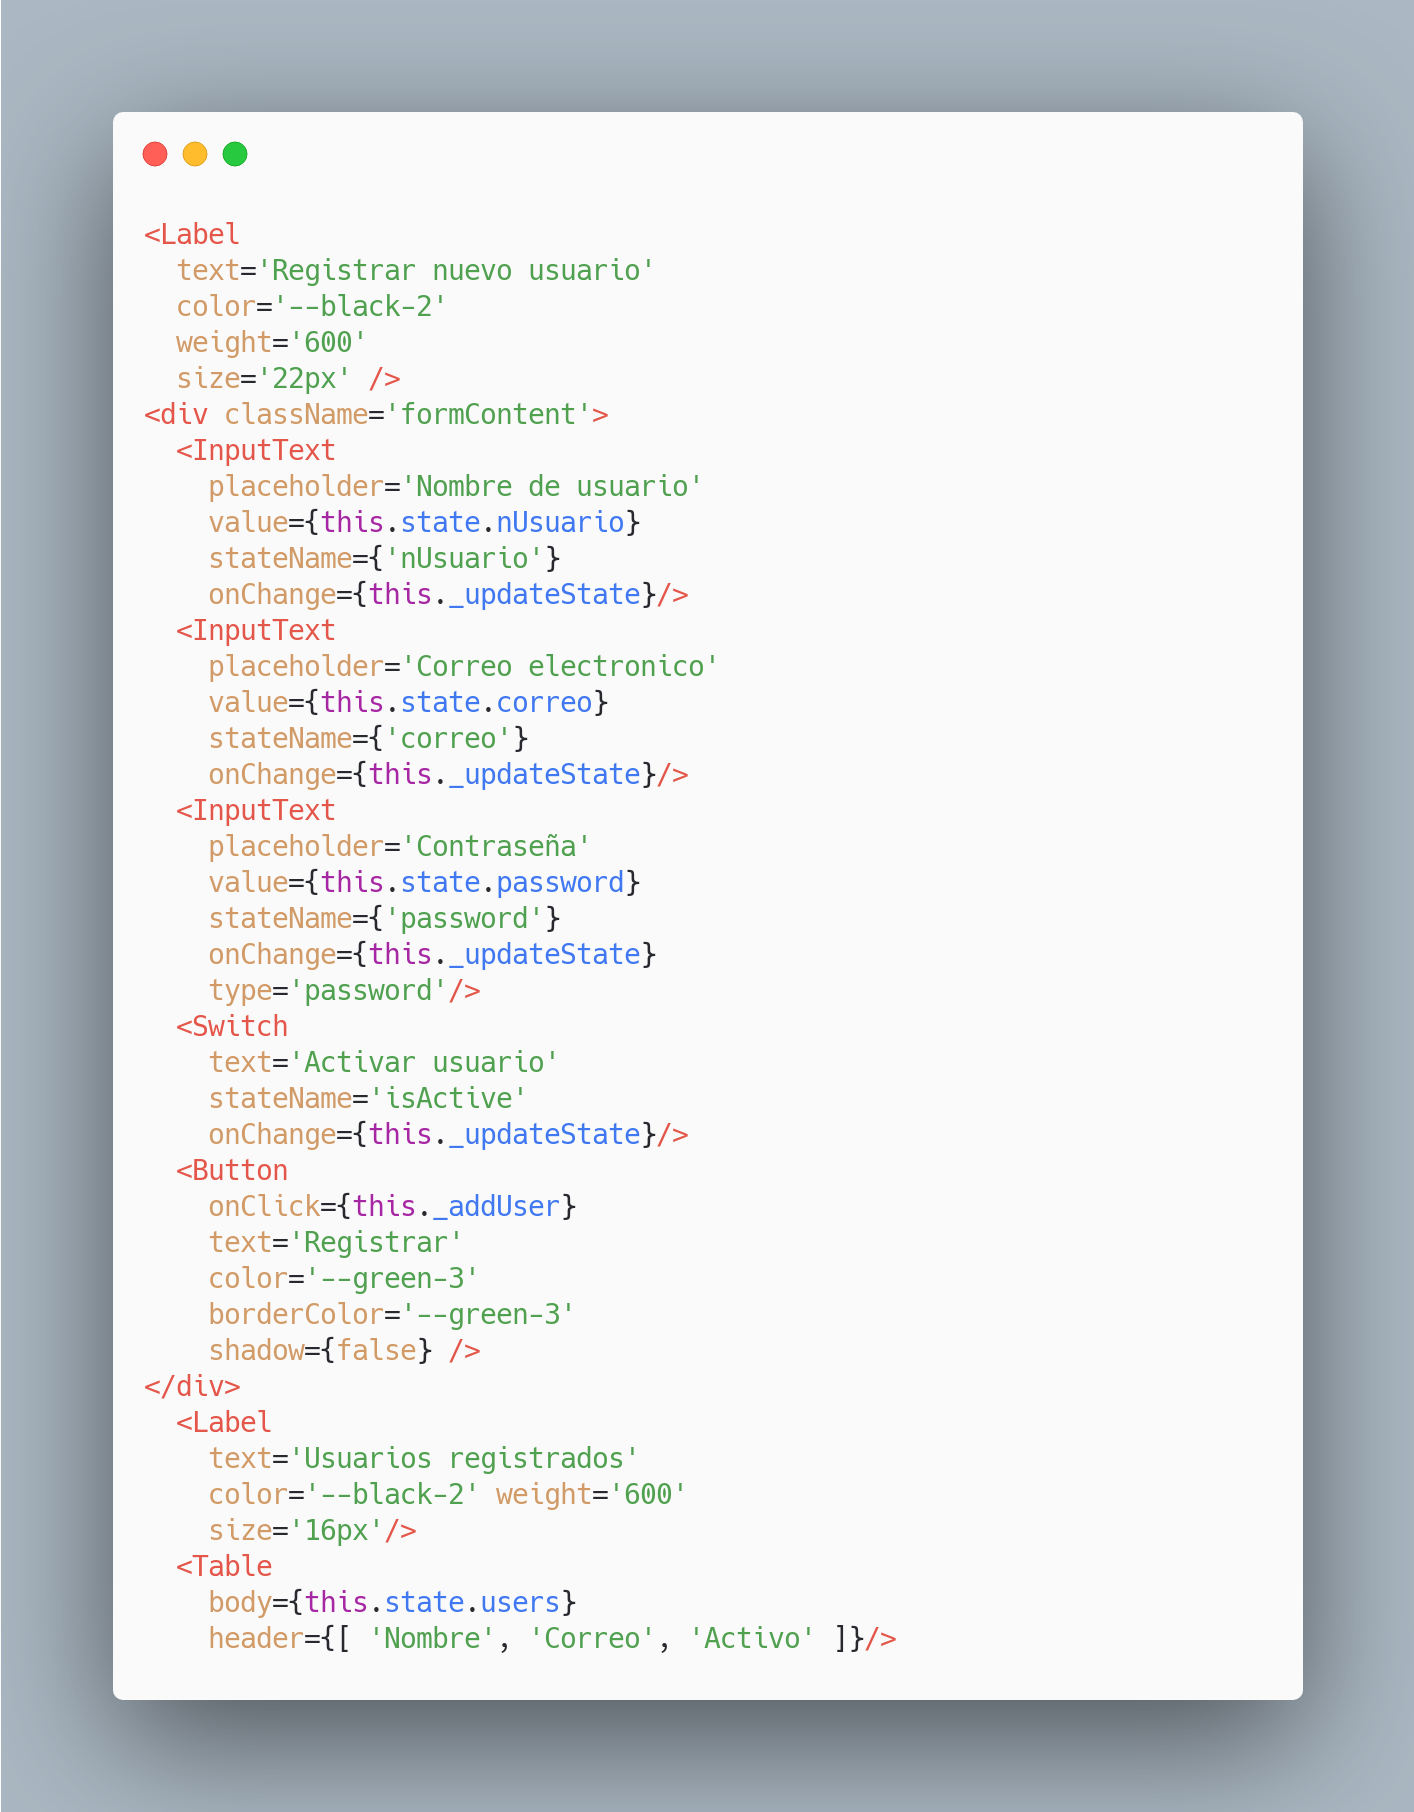
\includegraphics[width=1\textwidth]{./Imagenes/9.8}
   \centering 
    \caption[Código para maquetar]{Código para maquetar}
    \end{figure}
\newline

El código contiene al inicio un componente Label el cual muestra en pantalla un texto dado con las especificaciones de preferencia, se le da un tamaño de letra y color del texto. Después siguen una serie de InputText los cuales son la entrada de datos para el nombre de usuario, correo electronico  y contraseña, Estos tienen parámetros que son importantes de mencionar ya se son indispensables para el correcto funcionamiento como son:
placeholder: Es el texto que se mostrará en el campo de texto antes de que se introduzca un dato, para dar una pista del dato solicitado.
value: Es el estado de React en el que se almacenará cuando ocurra un cambio.
stateName: Es la forma en como es llamado en el estado de react ( Ejemplo. en este caso sería alguna de las llaves que se muestran en la Figura 9.6 ).
onChange: Es la función que se activará cuando algún dato se actualice.

El último parámetro onChange es una función simple como la que se muestra a continuación. 

\newline
\begin{figure}[H]
    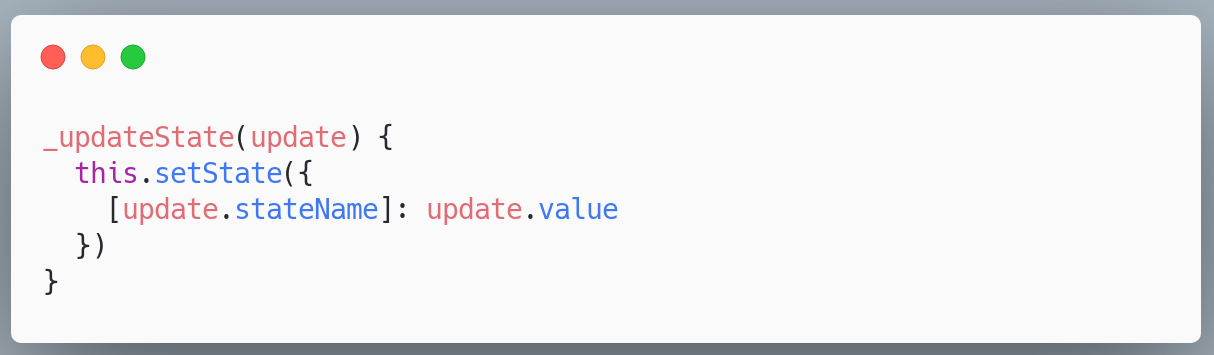
\includegraphics[width=1\textwidth]{./Imagenes/9.9}
   \centering 
    \caption[Función para actualizar el estado de React]{Función para actualizar el estado de React}
    \end{figure}
\newline

Esta función es única para cualquiera de los componentes de la librería, ya que están diseñados para que cuando se actualicen, regresen el nombre por el cual están identificados en el estado de React para saber que dato actualizar  y el nuevo valor.
Finalmente se tiene el componente Button y Table. El componente Button tiene un parámetro, onClick el cual envía una función que se ejecutará cuando se haga click. Esta función actualiza el parámetro del estado llamado users que almacena de manera no persistente los usuarios que se vayan agregando.
El componente Tabla recibe un arreglo para la cabecera y un arreglo de arreglos para el cuerpo de la tabla.


A continuación se muestra el resultado que se tendría con unas escasas líneas de código usando la librería.
\newline
\begin{figure}[H]
    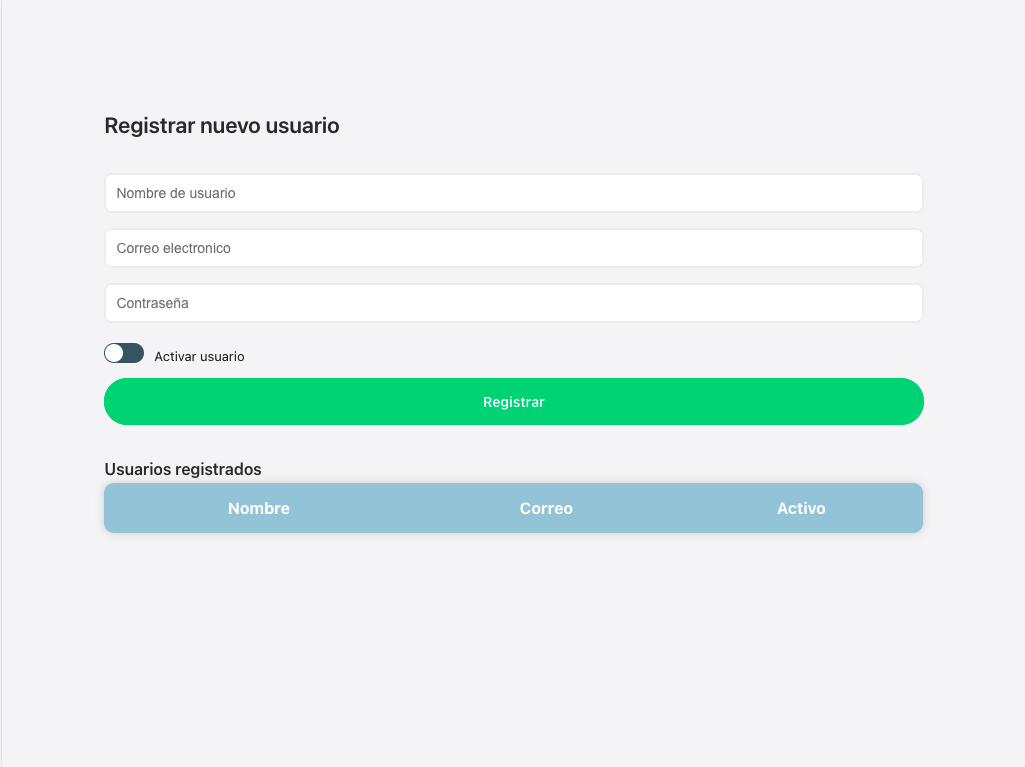
\includegraphics[width=1\textwidth]{./Imagenes/9.10}
   \centering 
    \caption[Resultado final]{Resultado final}
    \end{figure}
\newline
También se tiene el resultado después de agregar algunos usuarios.
\newline
\begin{figure}[H]
    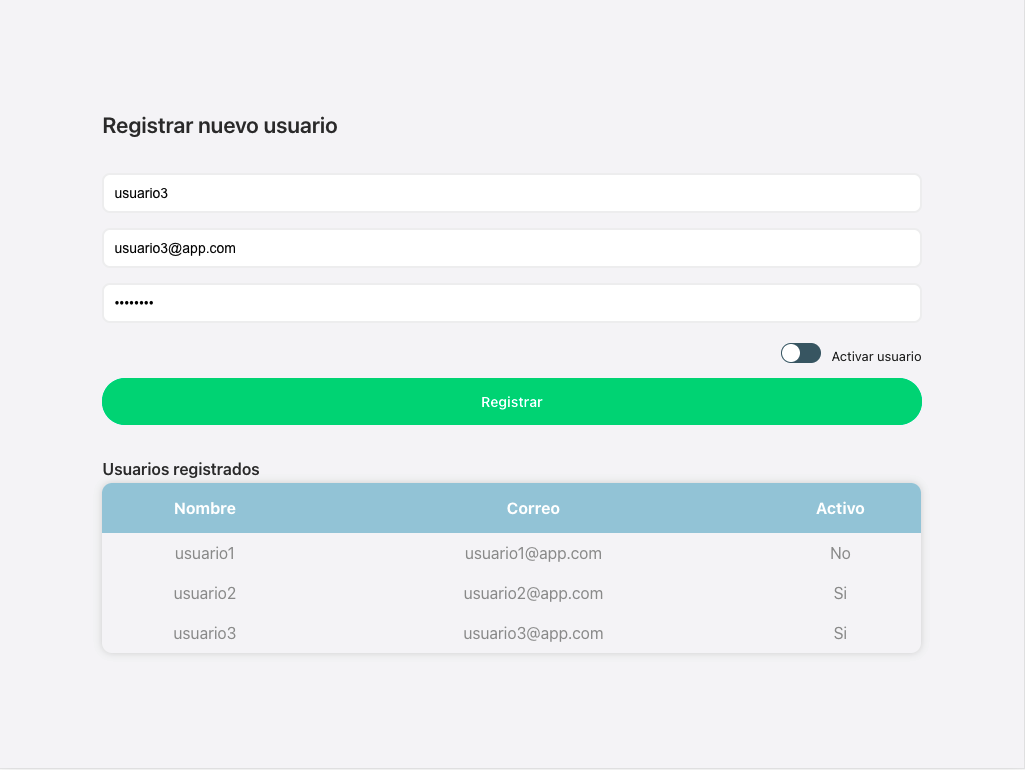
\includegraphics[width=1\textwidth]{./Imagenes/9.11}
   \centering 
    \caption[Resultado final al agregar usuarios]{Resultado final al agregar usuarios}
    \end{figure}
\newline

En seguida se muestra otro ejemplo que figura un restaurante en el cual se muestran los platillos que se venden, con la posibilidad de filtrarlos si son bebidas o tragos.

En el estado de React se tiene solamente un dato, este es el modo por el cual se están filtrando los datos.
\newline
\begin{figure}[H]
    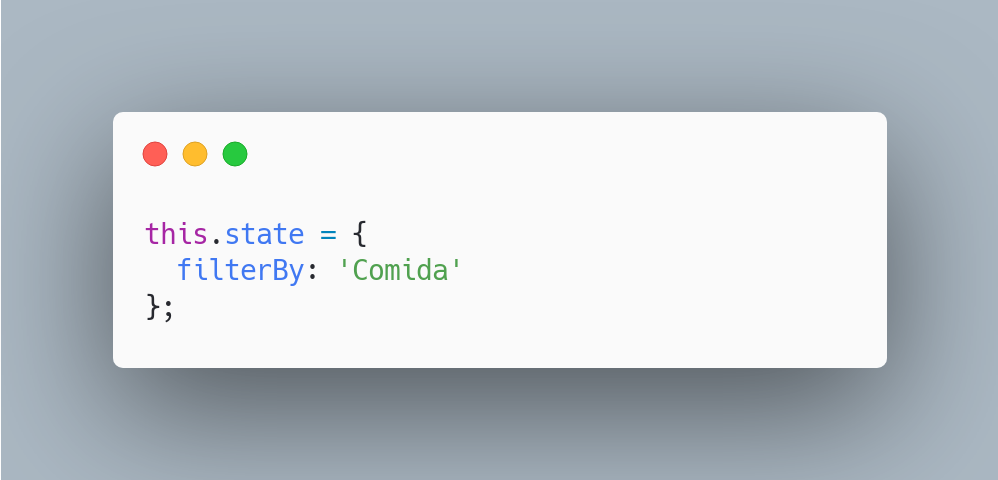
\includegraphics[width=0.7\textwidth]{./Imagenes/9.11-2}
   \centering 
    \caption[Filtro en el estado de React]{Filtro en el estado de React}
    \end{figure}
\newline

El código para maquetar los platillos es el siguiente el cual puede ser usado por ejemplo para la web de un restaurante la cual recibe los datos de algún otro servicio web.
El código de la siguiente web cuenta con elemento DropDown que permite filtrar para mostrar comida o tragos las opciones posibles para mostrar son enviadas por el parámetro options, stateName es el nombre de llave que almacena la opción por la que se filtra, y también se tiene optionSelected que es en si el filtro.

Después se tiene un ciclo en el que se agrega cada uno de los platillos, el componente Card recibe el título de la tarjeta, la imagen y el contenido.
\newline
\begin{figure}[H]
    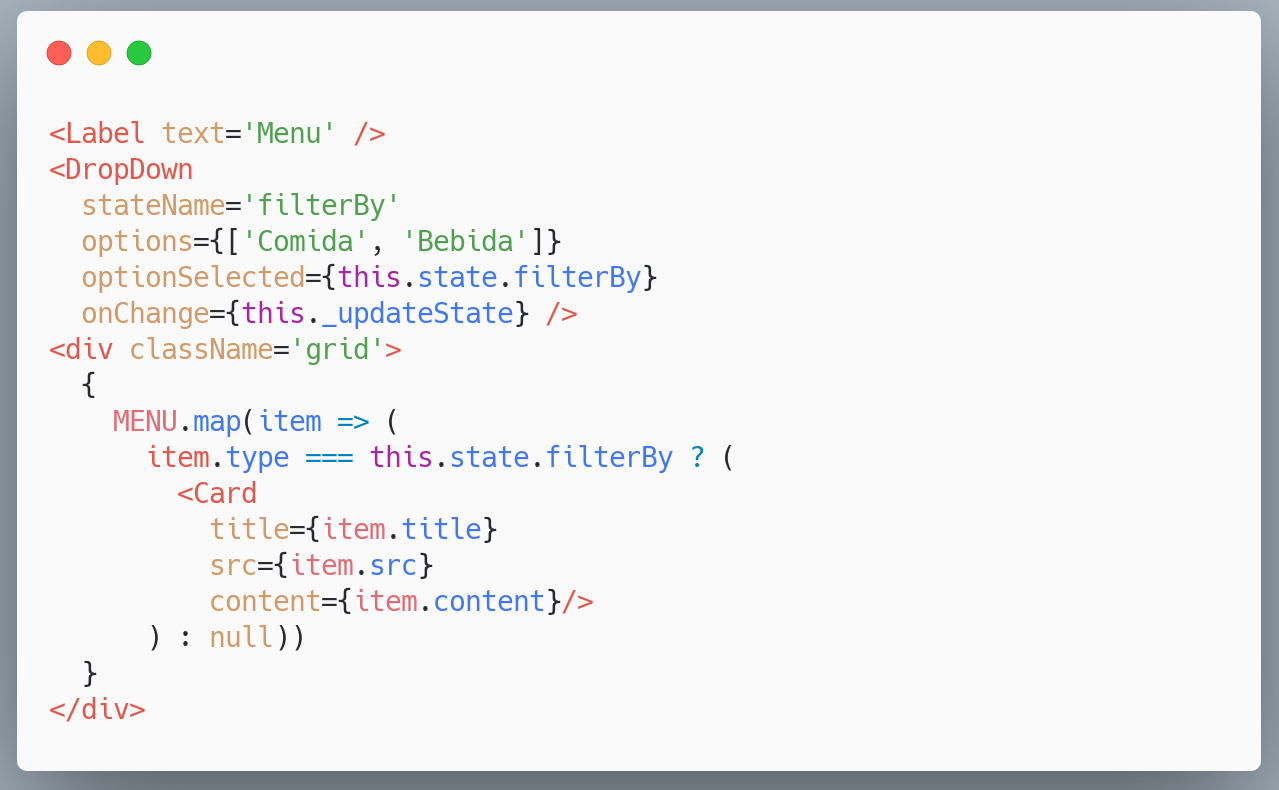
\includegraphics[width=1\textwidth]{./Imagenes/9.12.png}
   \centering 
    \caption[Código para mostrar los platillos]{Código para mostrar los platillos}
    \end{figure}
\newline

En las siguientes imágenes se muestra el resultado del código.
\newline
\begin{figure}[H]
    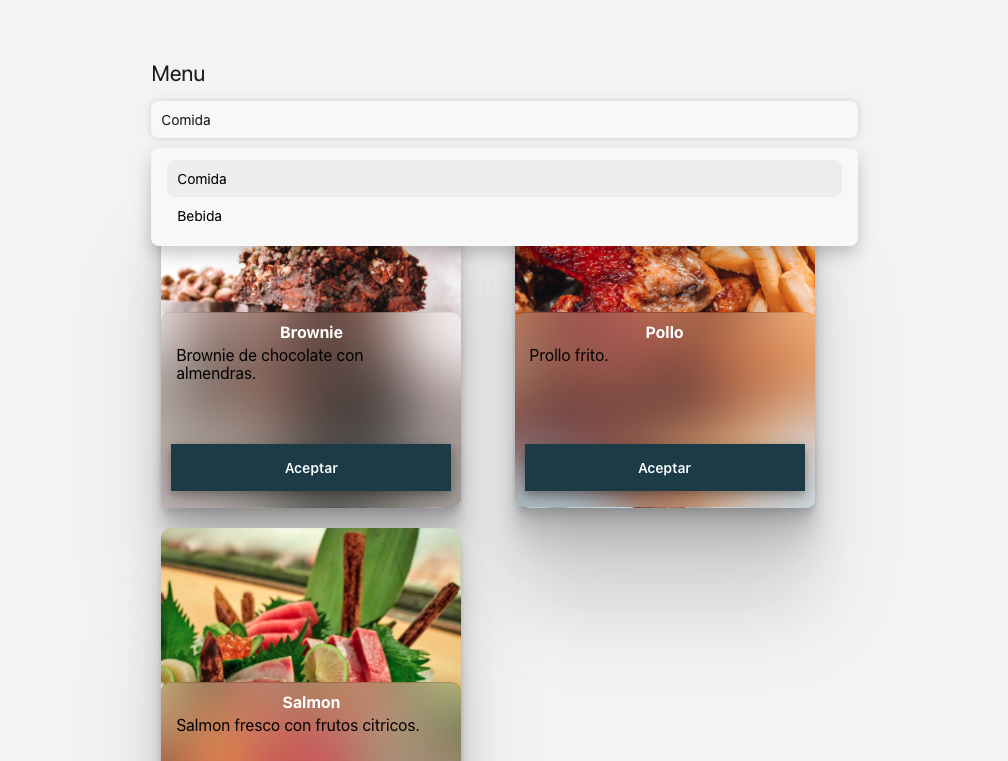
\includegraphics[width=1\textwidth]{./Imagenes/9.13.png}
   \centering 
    \caption[Filtrar por comida]{Filtrar por comida}
    \end{figure}
\newline

\newline
\begin{figure}[H]
    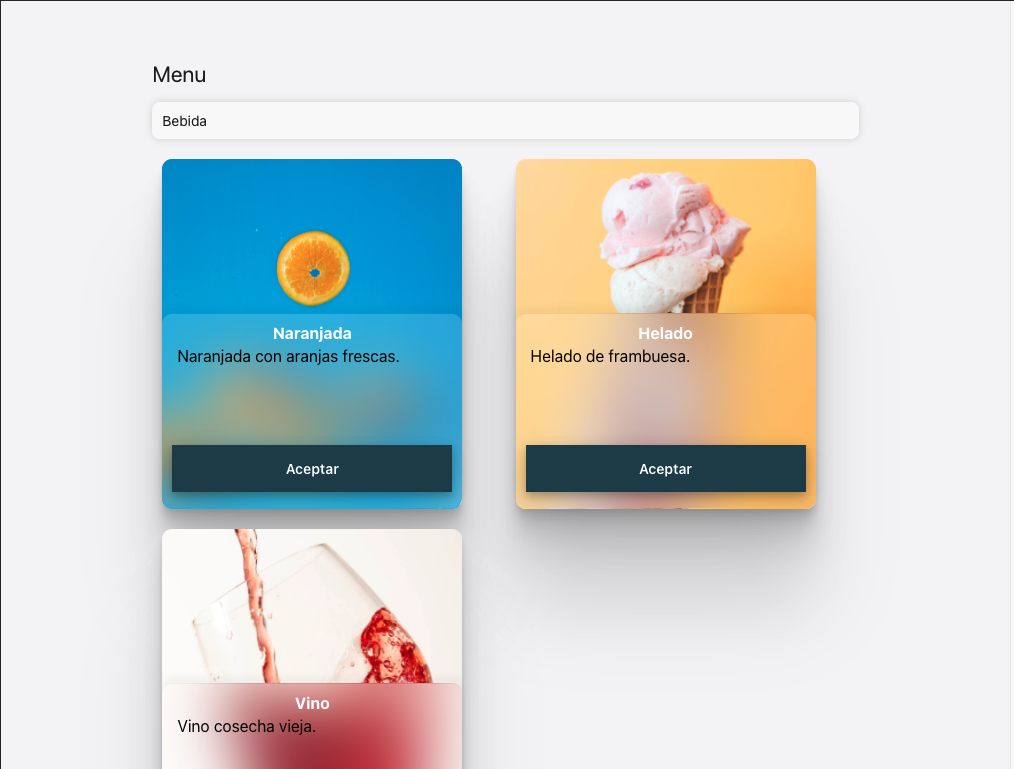
\includegraphics[width=1\textwidth]{./Imagenes/9.14.png}
   \centering 
    \caption[Filtrar por bebida]{Filtrar por bebida}
    \end{figure}
\newline

También se cuenta con el elemento Modal que puede ser usado como confirmación cuando el comprador presiona el botón para comprar un platillo.
\newline
\begin{figure}[H]
    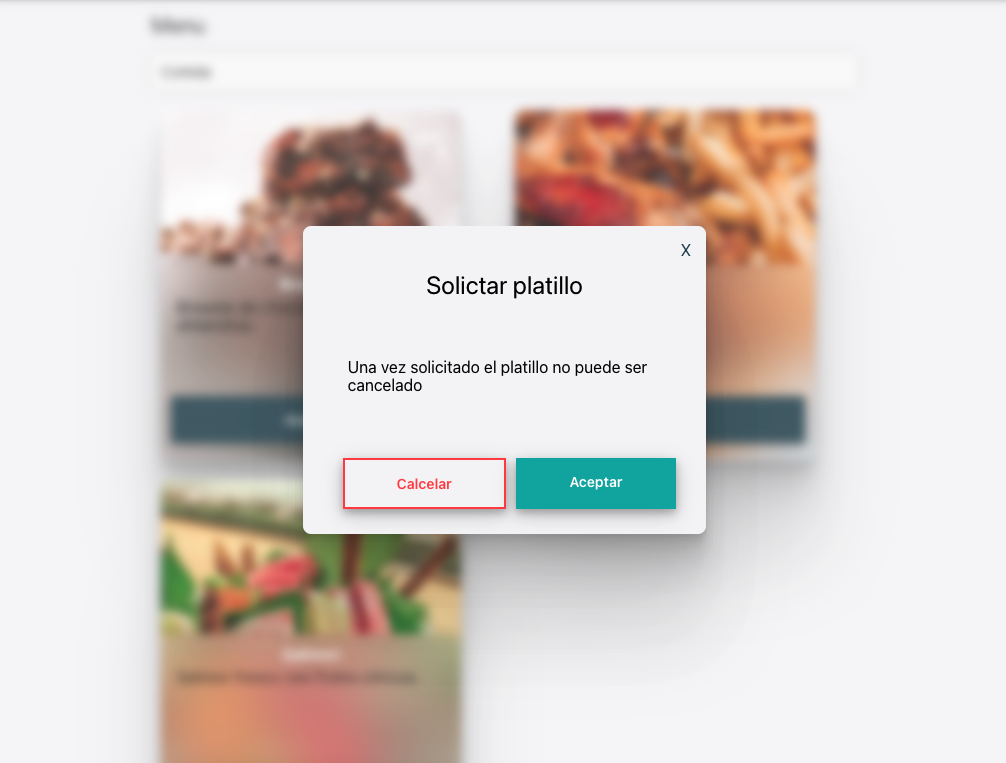
\includegraphics[width=1\textwidth]{./Imagenes/9.15.png}
   \centering 
    \caption[Confirmación de pedido]{Confirmación de pedido}
    \end{figure}
\newline

